\section{Method}
\label{sec:method}

The study design and analysis followed the guidelines set out by \citet{runeson_guidelines_2008}, and incorporate elements of human- and application-grounded evaluation~\cite{doshi2017towards}. Data was collected in parallel from two sources:

\begin{itemize}
    \item A structured online questionnaire, collecting quantitative results from a large number of respondents
    \item A series of semi-structured expert interviews, providing qualitative insights to triangulate and contextualize these results. 
\end{itemize}

\subsection{Questionnaire design}

The questionnaire was built as a web application in React.js with the SurveyJS framework \cite{devsoft-baltic-ou-2021}. The full survey code and can be found in the GitHub repository accompanying this paper~\footnote{https://github.com/theodore-evans/xai-in-digital-pathology}

% \cite{evans-2021}.

\subsubsection{Choice of sample AI output}

An AI-assisted Ki-67 quantification was chosen as a representative task from the slide examination step of the digital pathology workflow~\cite{Kargl-et-al:2020:PathoWorkflows}.

Ki-67 is most widely used cellular proliferation marker in pathology~\cite{li2015ki67}. It is an immunohistochemistry (IHC) stain that highlights the nuclei of cells that are preparing for, or already undergoing, cell division~\cite{scholzen2000ki}. In clinical diagnostic work, it is used to characterize many different neoplasms as well as non-neoplastic conditions~\cite{nadler2013ki}. The result may assist tumor classification and strongly impact treatment decisions. 

Quantifying Ki-67 positivity in a diagnostic setting exhibits a high degree of variance from both pre-analytical (laboratory) and analytical (pathologist) sources~\cite{polley2015international, rimm2019international}. Identification of AI-assistance as a promising means to mitigate variability has led to a Ki-67 analysis becoming one of the most common applications of AI assistance in pathology~\cite{geread2021pinet, lakshmi2020deep, govind2020improving}, with the first CE mark designations having been awarded for such an application~\cite{business-wire-2021}.  

Moreover, the type of model architecture suited to this task, semantic segmentation with thresholding and quantification, is well represented amongst those AI solutions already seeing market penetration in digital pathology, as evidenced by the awarding of FDA and/or EU CE-IVD approval~\cite{garcia2019new}. Therefore, study findings with respect to this type of model are more likely to be transferable to a wider range of other applications in digital pathology.

The sample output used as a basis for the explanations presented in this research was created using the PathoNet deep learning model, trained for 30 epochs on the SHIDC-BC-Ki-67 dataset using the developer-recommended hyperparameters \cite{negahbani2021pathonet}. The final sample output, shown in Figure~\ref{fig:exampleoutput}, was chosen arbitrarily from a selection generated by the demonstration script included in code repository accompanying this paper. The annotations were re-colored to a colorblindness-friendly red-blue color scheme, and an inset indicating the per-slide and per-region detected positivity was manually added, with figures derived from the model output.

\begin{figure}[!ht]
    \centering
    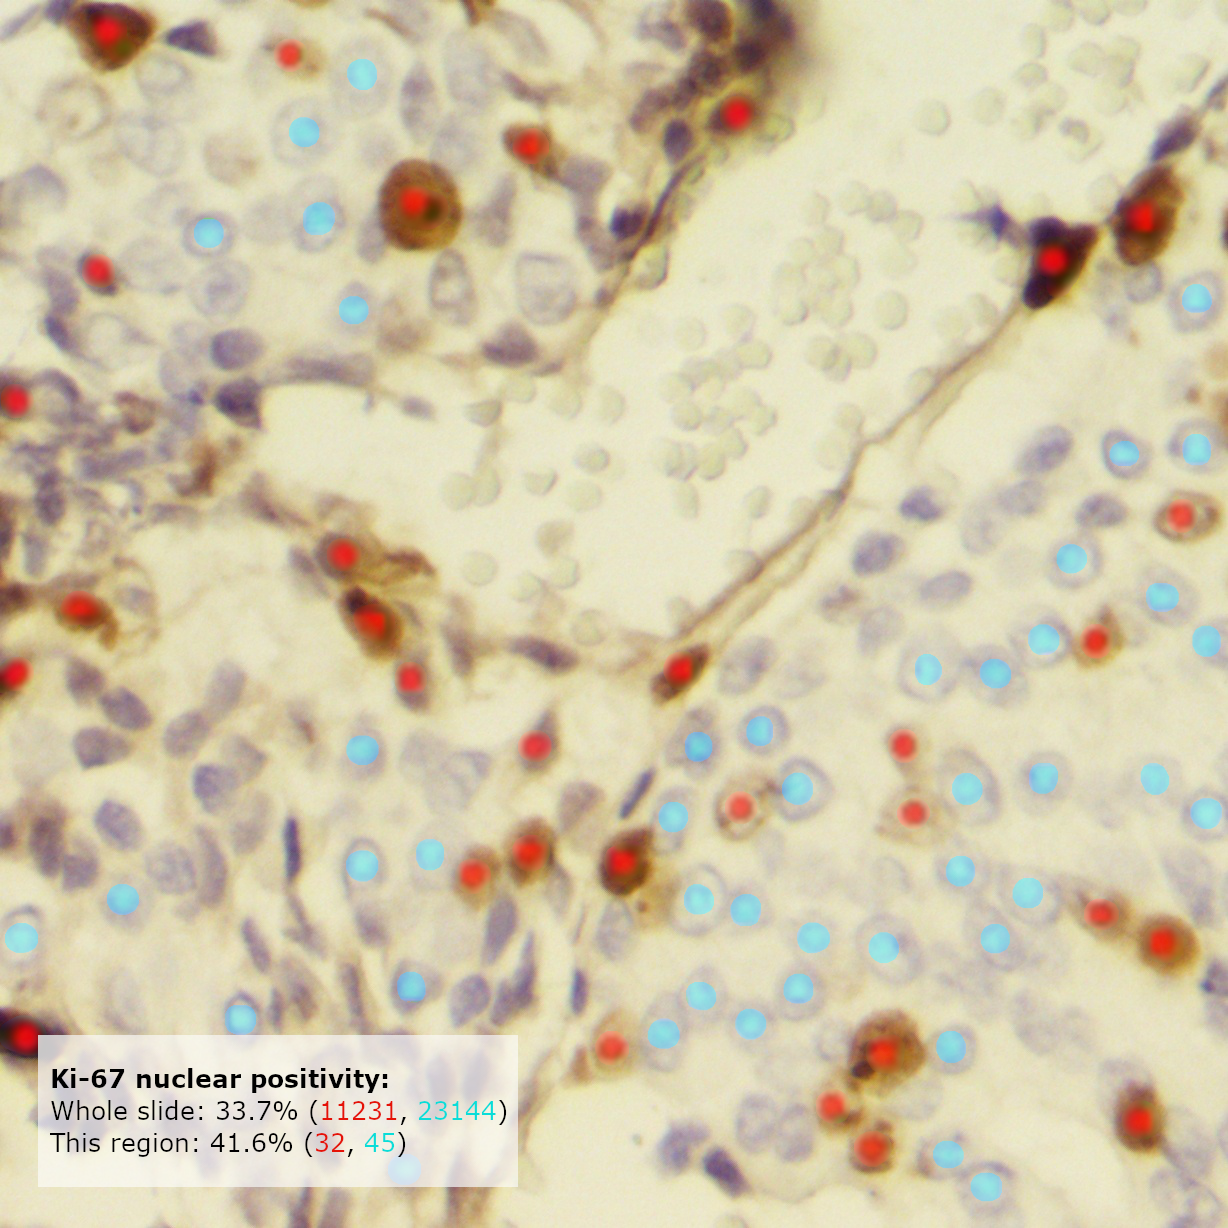
\includegraphics[width=0.85\linewidth]{Graphics/3CaseStudyDesign/base_image.png}
    \caption{The sample AI output showing nucleus annotations and overall Ki-67 quantification result.}
    \label{fig:exampleoutput}
\end{figure}

% The sample shows a region of interest from an IHC-stained biopsy slide from the SHIDC-B-Ki-67 dataset, overlaid with annotations generated by a Ki-67 detection algorithm~\cite{negahbani2021pathonet}, denoting positive and negative tumor nuclei in red and blue respectively. The overall positivity score is shown inset, simulating a snapshot from a typical computer-assisted Ki-67 grading task.

\subsubsection{Selection and Creation of Example Explanation}

In the main body of the questionnaire, respondents were presented with the sample output of a fictitious AI solution for assistance in detection and grading of Ki-67 nuclear positivity (Figure~\ref{fig:exampleoutput}). Each questionnaire page displayed an alternative example explanation of the sample AI output, with each explanation falling into one of five main classes representing the state of the art described in Section~\ref{sec:related:classes}.

Given their relative ease of implementation, \textbf{Saliency Map} examples were generated using real techniques from the state of the art, applied on the PathoNet model with Neuroscope~\cite{schorr_neuroscope_2021}, an xAI toolbox for deep learning-based segmentation models. The techniques used were guided backpropagation~\cite{springenberg2014striving} and Grad-CAM~\cite{selvaraju2017grad} with respect to the class output layer of the model. The Grad-CAM implementations were presented as both global (an overlay on the entire input region) and local (an overlay on a single nucleus) explanations. Each participant was shown both a global and local example.

The other explanation classes were mocked up with image processing software, based upon existing or hypothetical explainability approaches from the literature, and guided by feedback from pathologists at the Charité Berlin, as well as ML and medical AI experts at Fraunhofer MEVIS, Bremen, and the DAI-Labor, Technische Universität Berlin.

\textbf{Concept Attribution} examples were created based on the TCAV approach of \citet{kim2018interpretability}, such that the relative importance of a set of human-interpretable concepts to the positive model outcomes were displayed as an explanation for the overall AI output. Two variations were included, featuring alternative wording for the high-level concepts. 

\textbf{Prototypes} examples featured an inset image showing two nuclei that were marked in the Grad-CAM saliency map (as above) as most strongly relevant for the Ki-67 positive and negative classes, respectively.

\textbf{Counterfactual} examples were created based on a generative latent variable traversal approach similar like those of \citet{liu2019generative}. These were supplemented with manually decision boundaries and an additional implementation showing two axes of variation on one figure. The examples themselves were created by morphing between prototypical examples of positive, negative and unclassified nuclei using an open source tool~\cite{diffmorph:github}.

\textbf{Trust Scores} examples were created to represent the concept of per-annotation confidences, grouped into low- and high-confidence classes. These were created by intersecting the class activation Grad-CAM maps with the PathoNet classifications and using the aggregated per-pixel relevance over each nucleus as a proxy for per-annotation model confidence, grouping these in terms of high- and low- confidence.

To better represent the diversity of approaches, a number of example from each class was chosen to approximately reflect its prevalence in the literature. To mitigate the impact of potentially uninformative individual implementations, multiple image variants of selected instances were prepared where possible, with one of these displayed at random for each participant. 

A total number of seven examples to be displayed was chosen to limit the estimated questionnaire completion time to around five minutes. This time limit was chosen to minimise the risk of fatigue and participant dropout, particularly in light of the limited availability of the target audience. To reduce the impact of recency and primacy, explanation classes were displayed in random order, whilst keeping examples from the same class consecutive. The examples and their variants are shown in Figure~\ref{fig:classes_overview}.

\begin{figure*}
\centering
\begin{minipage}[c]{0.85\textwidth}
    \includegraphics[width=\linewidth]{main/Graphics/3CaseStudyDesign/xAI Classes Overview reordered.png}
    \caption{Explanation examples, along with their plain-text descriptions and image variants, as presented in the online questionnaire and face-to-face interviews. The figure is provided in high resolution and can be zoomed for a detailed view.}
    \label{fig:classes_overview}
\end{minipage}
\end{figure*}

\subsubsection{Rating questions}
 For each explanation, respondents expressed their degree of agreement, rated on a 7-point scale between \textit{Strongly disagree} and \textit{Strongly agree}, to each of four following statements:

 \begin{enumerate}
    \item I find the explanation intuitively understandable
    \item The explanation helps me to understand factors relevant to the algorithm
    \item The explanation helps me to decide whether I can trust the generated annotations
    \item The explanation provides me with valuable information for my work
\end{enumerate}

These statements were designed to gauge a measure of usability, similar to that targeted by the System Usability Scale (SUS)~\cite{brooke1996sus} and the xAI-oriented System Causability Scale (SCS) \cite{HolzingerEtAl:2020:QualityOfExplanations}, in a format appropriate for a short survey with multiple, non-interactive examples. The ordering was chosen to reflect a hierarchy of needs, whereby each subsequent item is unlikely to be highly rated unless there is a strong agreement on all previous statements, with the aim of reducing cognitive load without the need for explicit branching. A sample screenshot of the questionnaire is shown in Figure~\ref{fig:examplepage}.

 \begin{figure*}[ht]
    \centering
    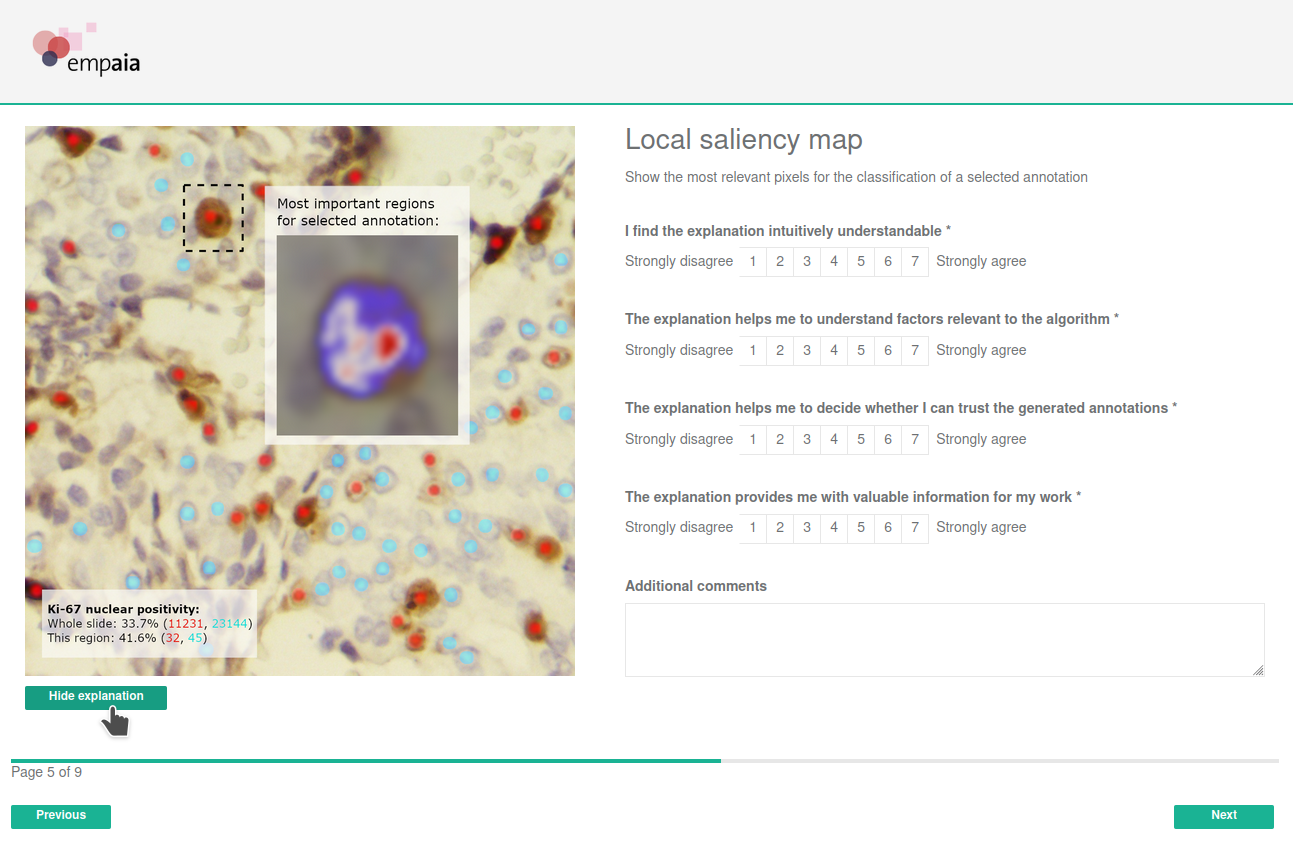
\includegraphics[width=0.75\linewidth]{Graphics/3CaseStudyDesign/example_page.png}
    \caption{An example explanation as presented to a participant. The sample AI output is overlaid with one of the possible explanation instances. Clicking on either the image or the \emph{Hide/Show explanation} toggles visibility of the explanation for A/B comparison. Each explanation is accompanied by a name and short plain-text description. The four Likert statements are shown on the right, with an optional comments field below.}
    \label{fig:examplepage}
 \end{figure*}
 
\subsubsection{User profiling}

The following information about each respondent was collected:

\begin{itemize}[noitemsep]
    \item Age
    \item Professional position
    \item Usage of digital pathology or telepathology
    \item Usage of AI solutions
    \item Familiarity with technical details of machine learning
    \item Familiarity with AI applications in pathology
\end{itemize}

These questions closely follow those posed in a user-profiling questionnaire to pathologists disseminated by the Medical University of Graz \cite{HolzingerEtAl:2021:PersonasToolbox}, to allow for cross-evaluation of these results in future work.

\subsubsection{Dissemination strategy}

The questionnaire was open to submissions between 11.06.2021 -- 26.07.2021, having been made public via Twitter on 11.06.2021 (@TheEMPAIA) and again on 15.07.2021 (@DAI\_Labor) and via the EMPAIA newsletter (14.07.2021).

\subsection{Expert interview design}
\label{sec:interviewdesign}
Expert interviews were conducted over video call with a semi-structured format, loosely following the structure of the online questionnaire. Following a short introduction to the outline, goals and purposes of the interview, including the collection of informed consent to begin recording, the interviewee was asked a few questions regarding their professional position, background and experience with AI applications in pathology. The interviewee was then shown the sample AI output in a simplified version of the online questionnaire, followed by the example explanations in a randomized order. Each interview lasted around one hour in total.

For each example, the interview was structured around a number of open-ended research questions: 

\begin{itemize}
    \item How do you interpret the explanation shown here?
    \item What does the explanation tell you about how the model is reaching this outcome?
    \item How does the explanation affect your trust in the model output?
    \item How might an explanation like this be valuable to you?
    \item What could make this type of explanation better?
    \item Are there other tasks for which this explanation might be equally or better suited?
\end{itemize}

Not every question was asked to every participant, and room was left for open-ended discussion with the possibility of branching off into more general ideas about explainability and AI applications in pathology.

\subsection{Results analysis}

The questionnaire data was processed using Python. The complete notebook and raw data can be found in the accompanying code repository.

The interviews were conducted via Zoom call, recorded with the participants' informed consent. These recordings were transcribed with the assistance of AI-based service Otter.ai~\cite{otterai-2021}. The recordings and transcripts were manually reviewed and structurally coded according to the explanation classes and guiding interview questions described above.